\subsection*{Questão 02}

\textit{O que é espectro de frequências de um sinal?}

\textbf{Resposta:}
O espectro não é sobre o tempo, mas sobre a decomposição.
É a representação de um sinal no \textbf{domínio da frequência},
mostrando as amplitudes de cada componente senoidal que compõe o sinal original.

\begin{center}
    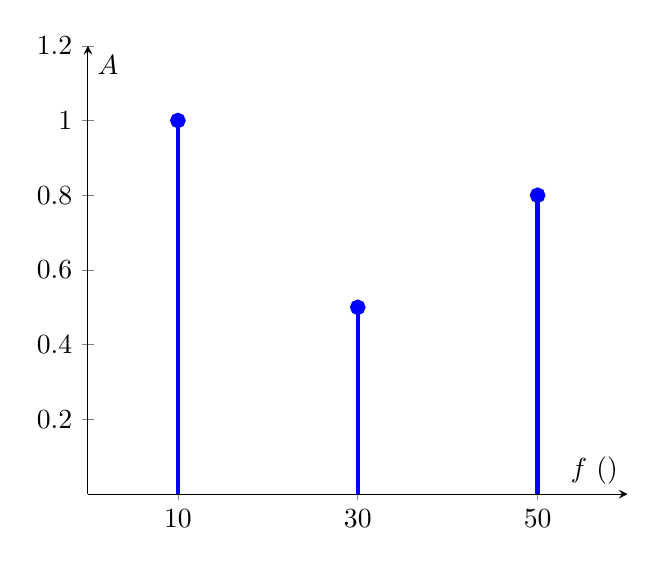
\begin{tikzpicture}
        \begin{axis}[
            ycomb,
            axis lines = middle,
            xlabel = $f$ (\khz), ylabel = $A$,
            xmin=0, xmax=60,
            ymin=0, ymax=1.2,
            xtick={10, 30, 50}
        ]
        \addplot 
            [blue, ultra thick, mark=*]
            coordinates {(10, 1) (30, 0.5) (50, 0.8)};
        \end{axis}
    \end{tikzpicture}
\end{center}